\chapter{Dasar Teori}

\section{\textit{Voice Assistant}}

\textit{Voice assistant}, atau asisten suara, merupakan turunan dari \textit{virtual assistant}. \textit{Virtual assistant} terdiri dari dua kata, \textit{virtual} dan \textit{assistant}. \textit{Assistant} atau asisten, menurut Kamus Besar Bahasa Indonesia, disingkat KBBI, adalah orang yang bertugas membantu orang lain dalam melaksanakan tugas profesional \parencite{kbbi}. Lalu \textit{virtual}, menurut KBBI, adalah tampil atau hadir dengan menggunakan perangkat lunak komputer. Jadi, dapat disimpulkan bahwa \textit{virtual assistant} adalah orang, dalam hal ini \textit{artificial intelligence}, yang hadir dalam sebuah perangkat tertentu, bertugas untuk membantu orang lain dalam melaksanakan tugas. \textit{Virtual assistant} kadang sering disebut dengan \textit{chatbot} karena kemampuannya dalam melakukan percakapan dengan penggunanya \parencite{tech2005imbot}. \textit{Virtual assistant} memiliki beberapa jenis interaksi selain melalui suara, seperti teks atau gambar. Salah satu jenis interaksi yang akan menjadi fokus dalam Tugas Akhir adalah interaksi melalui suara, atau disebut juga dengan asisten suara.

Gambaran besar mengenai \textit{voice assistant} dapat dilihat pada Gambar \ref{fig:slu_early} yang merupakan skema dari arsitektur awal pemahaman bahasa terucap atau \textit{spoken language understanding} \parencite{tur2011spoken}. Interaksi melalui suara pada dasarnya mirip seperti interaksi melalui teks, hanya saja perbedaannya terletak pada kemampuan asisten untuk melakukan \textit{speech recognition}. Asisten suara menggunakan teknologi pemahaman bahasa alami atau \textit{natural language understanding} (NLU) untuk mengolah suara yang diucapkan oleh pengguna menjadi kalimat lalu menemukan maksud pengguna melalui kalimat tersebut. Perlu diketahui bahwa \textit{speech recognition} dan NLU sama-sama memiliki sumber pengetahuan atau \textit{knowledge source}. Setelah asisten dapat "memahami" apa yang diucapkan oleh pengguna, asisten kemudian melakukan serangkaian aksi yang berkaitan dengan maksud ucapan pengguna tersebut.

\begin{figure}[H]
	\centering
	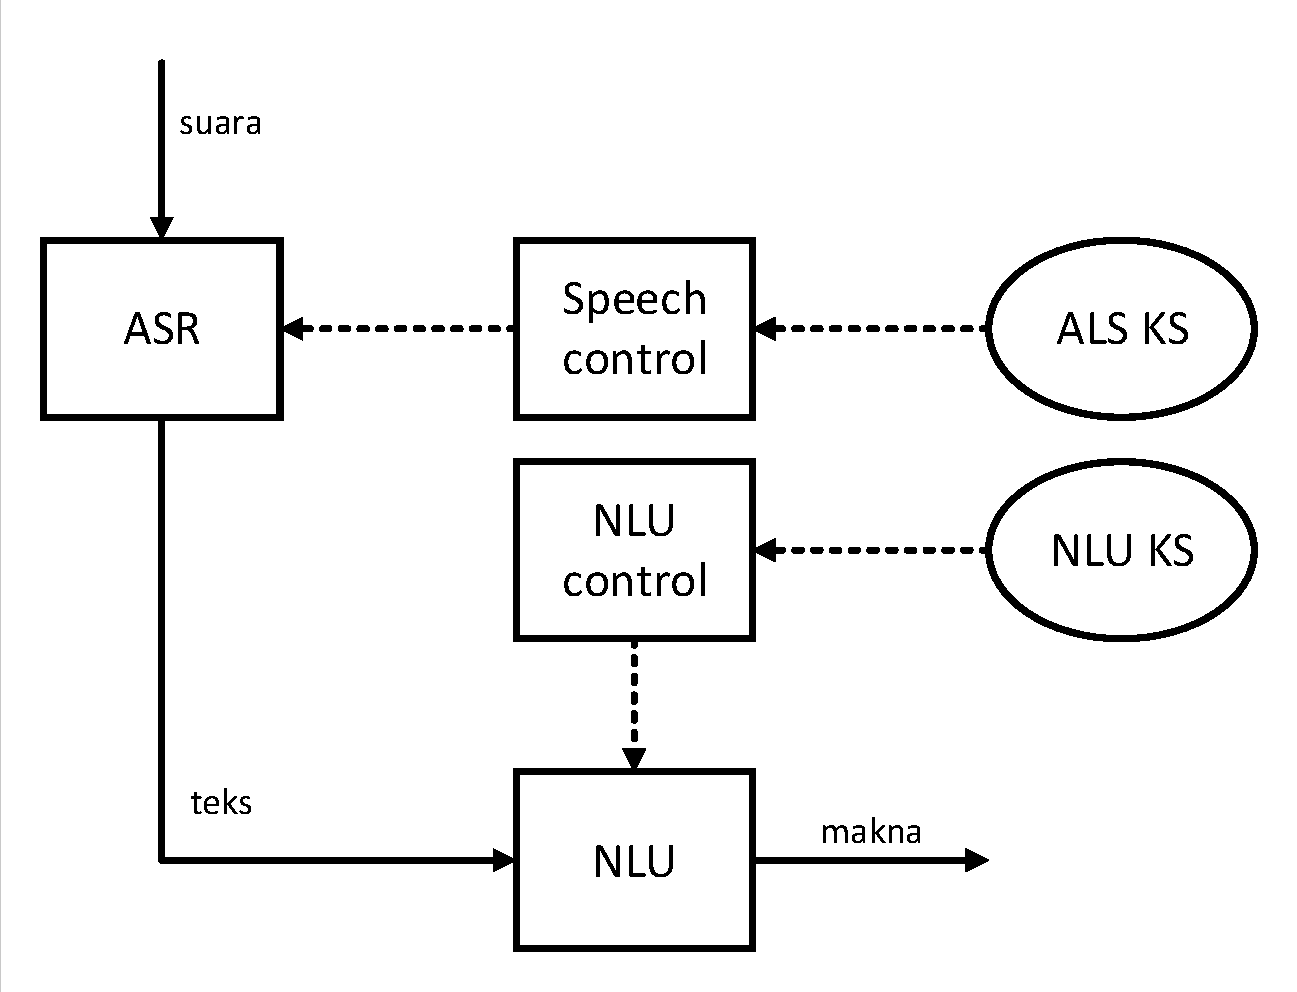
\includegraphics[width=0.5\textwidth, trim=2 2 2 2, clip]{resources/2/early_slu.pdf}
	\caption{Rancangan awal sistem SLU \parencite{tur2011spoken}}
	\label{fig:slu_early}
\end{figure}

Bagian \textit{voice assistant} yang menjadi fokus dalam pengerjaan Tugas Akhir adalah bagian NLU. NLU merupakan ranah dalam linguistik komputasional yang didedikasikan untuk memahami bahasa alami \parencite{harris2004voice}. Gartner mendefinisikan NLU sebagai pemahaman komputer terhadap struktur dan makna dari bahasa manusia sehingga pengguna dapat berinteraksi dengan komputer menggunakan bahasa yang digunakan oleh pengguna \parencite{gartnernatural}. Dari kedua definisi tersebut, dapat disimpulkan bahwa NLU merupakan bagian komputasional untuk memahami bahasa yang sering digunakan oleh manusia.

Perlu diperhatikan bahwa komputer berusaha untuk memahami bahasa manusia sehingga komputer perlu memiliki pengetahuan yang dasarnya dimiliki oleh manusia dalam berbahasa. James Allen menyebutkan bahwa terdapat enam bentuk pengetahuan yang diketahui dan dipelajari oleh manusia \parencite{allen1995natural}. Pengetahuan tersebut didefinisikan sebagai berikut:

\begin{enumerate}
	\item pengetahuan fonetik dan fonologi, menyangkut pada bagaimana suara diubah menjadi susunan kata-kata. Dalam ilmu komputer, pengetahuan ini diatasi dengan menggunakan \textit{speech recognition},
	\item pengetahuan morfologi, menyangkut pada bagaimana sebuah kata disusun dari beberapa morfem, seperti kata “terabaikan” disusun oleh tiga morfem, yaitu “ter-”, “abai”, dan “-kan”,
	\item pengetahuan sintaktis, menyangkut pada bagaimana kata-kata dapat disusun sehingga menjadi sebuah kalimat yang benar menurut tata bahasa,
	\item pengetahuan semantik, menyangkut bagaimana makna dari kata-kata disusun untuk membentuk makna dari sebuah kalimat,
	\item pengetahuan pragmatik, menyangkut bagaimana sebuah kalimat diartikan jika digunakan dalam konteks yang berbeda, dan,
	\item pengetahuan dunia, menyangkut memahami pengetahuan umum yang dipahami juga oleh pengguna untuk menjaga percakapan berjalan dengan semestinya.
\end{enumerate}

Pengetahuan yang dicakup dalam NLU saja adalah pengetahuan sintaksis, semantik, dan pragmatik. Terdapat empat kategori pendekatan yang digunakan untuk membangun NLU \parencite{yao2017four}. Pendekatan tersebut dijelaskan sebagai berikut:

\begin{enumerate}
	\item pendekatan distribusi, menggunakan taktik statistik skala besar dengan pembelajaran mesin (\textit{machine learning}),
	\item pendekatan berdasarkan rangka, menggunakan struktur data untuk representasi situasi yang sering terjadi,
	\item pendekatan model teoritis, menganggap sebuah kalimat selalu mengacu kepada yang ada di dunia dan bagian-bagian kalimat dapat digabungkan untuk membentuk sebuah makna, dan,
	\item pendekatan pembelajaran interaktif, menggunakan lingkungan interaktif antara manusia dengan komputer.
\end{enumerate}

Pendekatan yang menjadi fokus dalam pengerjaan Tugas Akhir adalah pendekatan distribusi, yang mana menggunakan pembelajaran mesin. Pembelajaran mesin adalah sebuah program komputer yang dirancang untuk belajar dari pengalaman \textit{E} dengan acuan berupa kelas tugas-tugas \textit{T} dan pengukuran performa \textit{P}, jika performa pada suatu tugas \textit{T}, yang diukur dengan \textit{P}, dan diperbaiki dengan pengalaman \textit{E} \parencite{mitchell1997machine}. Sebagai contoh, program menjalankan tugas (\textit{T}) untuk bermain dam. Ukuran program tersebut (\textit{P}) adalah persentase sebuah program menang dalam permainan dam. Untuk meningkatkan persentase tersebut, program harus belajar dari pengalaman (\textit{E}) berupa permainan yang telah dilakukan melawan program itu sendiri.

Terdapat tiga kategori umum untuk pembelajaran mesin berdasarkan cara belajar \parencite{ray2015essentials}. Tiga kategori tersebut adalah pembelajaran terkontrol, pembelajaran tidak terkontrol, dan pembelajaran penguatan. Algoritme pembelajaran terkontrol mengandung variabel terikat atau keluaran yang akan diprediksi jika diberikan sekumpulan variabel bebas sehingga membentuk fungsi yang dapat memetakan masukan menjadi keluaran yang diinginkan. Algoritme pembelajaran tidak terkontrol tidak memiliki variabel terikat untuk diprediksi sehingga algoritme harus mengelompokkan sendiri. Pembelajaran tidak terkontrol biasa digunakan untuk pengelompokan populasi ke dalam kelompok yang berbeda. Terakhir, algoritme pembelajaran penguatan menggunakan teknik coba-coba sebagai metode pembelajaran sehingga dapat membentuk program dengan keputusan yang spesifik. Algoritme yang menjadi fokus dalam Tugas Akhir adalah algoritme pembelajaran terkontrol, yang mana terdiri dari \textit{Nauve Bayes}, \textit{Decision Tree}, \textit{Support Vector Machine} (SVM), dan \textit{Artificial Neural Network} (ANN).

ANN adalah sistem komputasi yang memiliki elemen-elemen pemrosesan sederhana yang saling terhubung, yang mana dapat memproses informasi dengan respon keadaan dinamisnya kepada masukan dari luar \parencite{caudill1987neural}. Rupa ANN yang paling dasar dapat dilihat pada Gambar \ref{fig:ann} yang hanya terdiri dari tiga bagian lapisan, yaitu lapisan masukan, lapisan tersembunyi, dan lapisan keluaran. Satu lapisan terdiri dari kumpulan beberapa neuron yang digunakan sebagai fungsi aktivasi, dan neuron antar lapisan dihubungkan dengan bobot yang didefinisikan saat latihan berlangsung.

\begin{figure}[H]
	\centering
	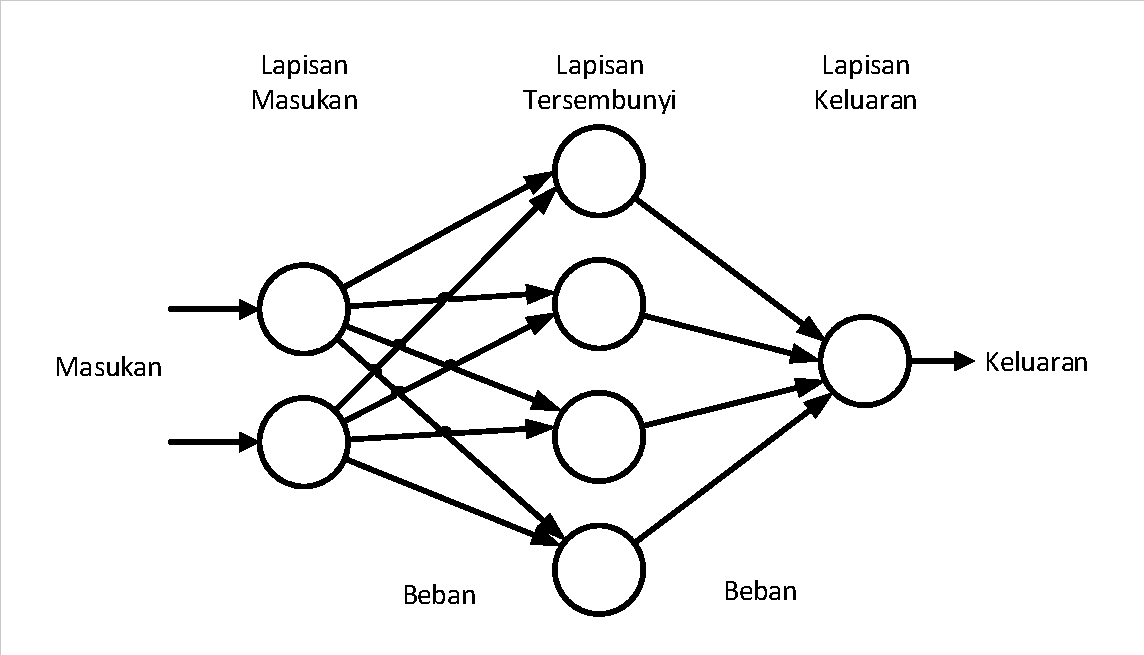
\includegraphics[width=0.8\textwidth, trim=2 2 2 2, clip]{resources/2/ann.pdf}
	\caption{Rupa dasar ANN}
	\label{fig:ann}
\end{figure}

Salah satu penerapan ANN untuk NLU adalah penggunaan lapisan \textit{embedding}, yaitu lapisan yang digunakan untuk membuat nilai vektor untuk tiap kata yang terlibat dalam pelatihan, dalam hal ini kata-kata yang ada di dalam kamus. Terdapat dua pendekatan \textit{embedding} yang digunakan untuk NLU, yaitu dengan menggunakan model bahasa yang telah dilatih dengan ukuran yang sangat besar atau mendefinisikan sendiri dengan menggunakan lapisan ANN. Pendekatan yang digunakan untuk pengerjaan Tugas Akhir adalah \textit{embedding} dengan menggunakan lapisan ANN.

Pengelompokan dilakukan dengan memasukkan lapisan \textit{embedding} dengan kata dalam bentuk tas kata (\textit{bag-of-words}). Tas kata dibentuk dari sebuah matriks satu dimensi, berisi nilai 1 untuk kata yang sesuai dan 0 untuk kata yang tidak sesuai. Untuk membentuk tas kata, sebuah kata diubah terlebih dahulu menjadi sebuah indeks. Pengubahan tersebut dilakukan dengan bantuan kamus.

Namun, terdapat permasalahan terhadap kamus yang dibentuk, salah satunya adalah kata yang akan diubah menjadi indeks harus ada di dalam kamus. Meskipun dalam kamus tersebut terdapat indeks khusus yang menyatakan kata yang tidak diketahui, namun kata tidak dapat diubah menjadi indeks kata yang tidak diketahui. Oleh karena itu, diperlukan salah satu fungsi yang dipasangkan sebelum menjadi masukan pada lapisan \textit{embedding}. Fungsi tersebut harus dapat menemukan kata dalam kamus yang mirip dengan kata yang sedang diubah menjadi indeks. Metode yang dapat digunakan untuk mencari kata yang mirip dalam kamus adalah dengan menggunakan metode jarak perbedaan antara kedua kata.

Jarak perubahan adalah jumlah operasi perubahan terkecil yang dibutuhkan untuk mengubah teks, misal teks A menjadi teks B \parencite{schutze2008introduction}. Terdapat beberapa variasi metode untuk mencari jarak perubahan kedua teks. Metode yang paling dikenal dalam jarak perubahan adalah dengan menggunakan jarak Levenshtein.

\section{Jarak Levenshtein}

Jarak Levenshtein, diciptakan oleh Vladimir Levenshtein, adalah jarak yang tercipta antara kedua teks atau kumpulan karakter yang dibandingkan. Jarak yang dihitung berdasarkan perubahan sebuah kumpulan karakter dengan kumpulan karakter yang lain, seperti penambahan, pengurangan, atau penggantian karakter \parencite{levenshtein1966binary}. Secara matematis, jarak Levenshtein kedua teks, $a$ dan $b$ dengan panjang masing-masing $|a|$ dan $|b|$, didefinisikan dengan $\text{lev}_{a,b}(|a|,|b|)$ yang mana:
\begin{equation}
	\text{lev}_{a,b}(i,j)=\begin{cases}
		\text{max}(i,j) & \text{ jika min} (i,j)=0, \\ 
		\text{min}\begin{cases}
			\text{lev}_{a,b}(i-1,j)+1\\ 
			\text{lev}_{a,b}(i,j-1)+1\\ 
			\text{lev}_{a,b}(i-1,j-1)+1_{(a_{i}\neq b_{j})}
		\end{cases} & \text{ selainnya}
	\end{cases}
\end{equation}
\myequations{Persamaan Jarak Levenshtein}
\noindent
dengan $1_{(a_{i}\neq b_{j})}$ adalah fungsi indikator yang bernilai 0 jika $(a_{i} = b_{j})$ dan sebaliknya, dan $\text{lev}_{a,b}(i,j)$ adalah jarak Levenshtein untuk $i$ karakter pertama pada teks $a$ dengan $j$ karakter pertama pada teks $b$. Sebagai catatan, ketiga persamaan yang berada dalam fungsi min menunjukkan ketiga operasi dari jarak Levenshtein. Persamaan pertama menunjukkan penambahan karakter, persamaan kedua menunjukkan pengurangan karakter, dan persamaan ketiga menunjukkan operasi penggantian karakter jika karakter yang dibandingkan tidak sama.

Jarak Levenshtein diaplikasikan untuk pengoreksi kata, sebagai contoh pemeriksaan ejaan. Dengan kemampuan untuk memeriksa ejaan, jarak Levenshtein dapat digunakan untuk melakukan normalisasi kata atau teks.

\section{Normalisasi Teks}

Terdapat sebuah penelitian terkait normalisasi teks. Penelitian tersebut berupa penelitian normalisasi teks dalam suntingan media sosial Twitter, atau disebut juga dengan \textit{tweet}, untuk bahasa Indonesia yang memiliki karakteristik berupa kata yang disingkat \parencite{saragih2017normalisasi}. Penelitian dilakukan oleh Tri Sony Saragih dengan tujuan untuk menerapkan algoritme penghitungan jarak dua kata dan membuat fungsi untuk normalisasi kata yang tidak baku menjadi kata baku. Keseluruhan pembangunan tersebut dilakukan dengan menggunakan bahasa pemrograman R.

Penelitian dilakukan dengan menggunakan fungsi \textit{stringdist} pada bahasa R. Fungsi \textit{stringdist} memiliki dua parameter wajib, yaitu kata pertama dan kata kedua, serta delapan parameter opsional, salah satunya adalah metode pengukuran jarak. Fungsi \textit{stringdist} memiliki 10 variasi metode pengukuran sebagai berikut:

\begin{enumerate}
	\item jarak \textit{optimal string alignment} (\textit{osa}),
	\item jarak Levenshtein (\textit{lv}),
	\item jarak \textit{full Damerau-Levenshtein} (\textit{dl}),
	\item jarak Hamming (\textit{hamming}),
	\item jarak \textit{longest common substring} (\textit{lcs}),
	\item jarak \textit{q-gram} (\textit{qgram}),
	\item jarak \textit{cosine} (\textit{cosine}),
	\item jarak Jaccard (\textit{jaccard}),
	\item jarak Jaro-Winker (\textit{jw}), dan,
	\item jarak \textit{Soundex} (\textit{soundex}).
\end{enumerate}

\subsection{Alur Proses Normalisasi}

Alur proses normalisasi teks yang dibangun dapat dilihat pada Gambar \ref{fig:flow_saragih}. Alur tersebut merupakan alur untuk tiap kata yang terdapat dalam \textit{tweet} berbahasa Indonesia. Proses membutuhkan dua jenis kamus, yaitu kamus kata tidak baku beserta perbaikannya dan kamus kata baku. Kamus kata tidak baku disusun dengan manual, yaitu dengan menentukan kata yang termasuk kata tidak baku bahasa Indonesia, baik kata dari bahasa daerah, bahasa gaul, atau bahasa asing, lalu menentukan kata baku yang merupakan makna dari kata tidak baku tersebut. Untuk kamus kata baku, terdapat tiga jenis kamus yang digunakan, yaitu kamus kata baku dari KBBI diambil dari sebuah perangkat lunak, kamus yang diambil dari korpus arsip situs web Kompas tahun 2012, serta kamus dari korpus Kompas yang telah disaring sehingga hanya mengandung kata yang sesuai dalam KBBI.

Proses normalisasi teks dimulai dari menerima kata masukan, lalu dilanjutkan dengan memeriksa kata masukan dengan kamus kata tidak baku. Jika kata masukan terdapat dalam kamus kata tidak baku, maka kata baku yang menjadi perbaikannya dipilih menjadi kata luaran. Jika tidak ditemukan, proses berlanjut dengan memeriksa kata masukan dengan kamus kata baku. Jika ditemukan, maka kata yang dipilih dalam kamus kata baku tersebut menjadi kata luaran. Jika tidak, proses dilanjutkan dengan mencari kata yang mirip di dalam kamus kata baku dengan menerapkan fungsi \textit{stringdist}.

Fungsi \textit{stringdist} digunakan untuk mencari jarak minimum antara kata masukan dan kata dalam kamus kata baku. Setelah itu, jarak minimum tersebut digunakan untuk mencari kumpulan kata dalam kamus kata baku. Jika hanya ditemukan satu kata dalam kamus, maka kata tersebut yang terpilih menjadi kata luaran. Jika ditemukan lebih dari satu, maka kata dalam kamu yang dipilih menjadi kata luaran adalah kata yang pertama kali ditemukan. Metode tersebut dipilih dengan mempertimbangkan bahwa kata dalam kamus yang berasal dari korpus Kompas diurut berdasarkan frekuensi kemunculan kata tersebut.

\begin{figure}[H]
	\centering
	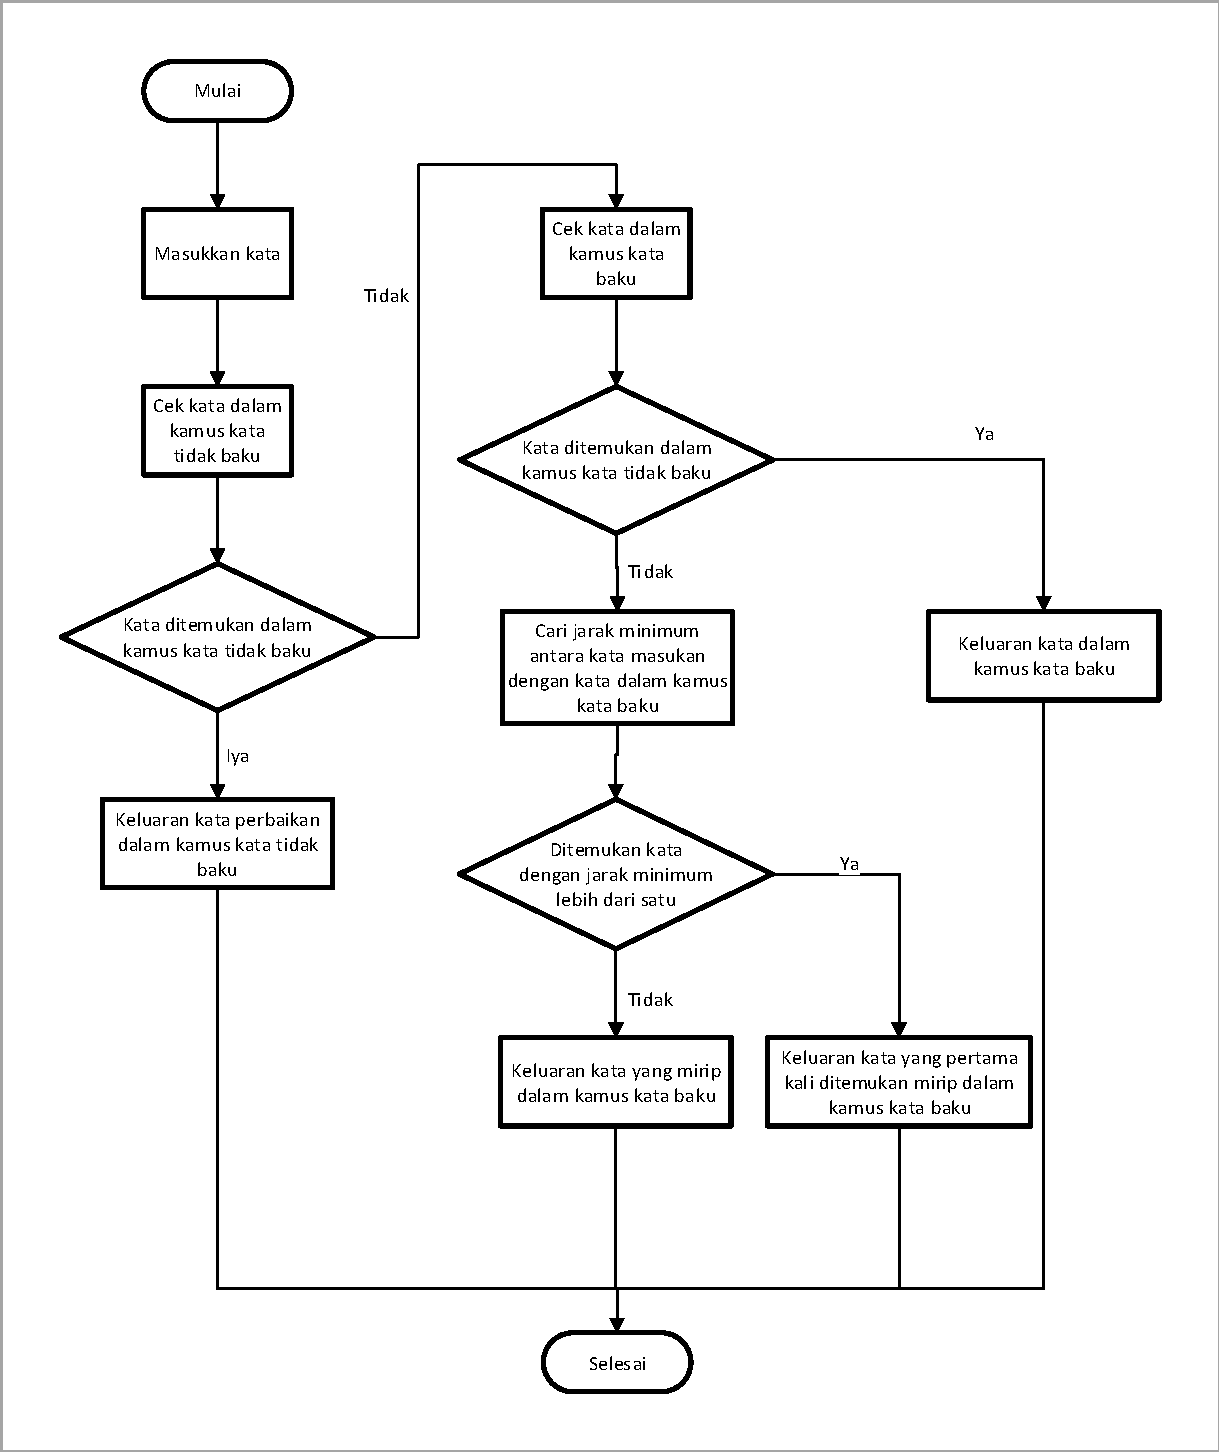
\includegraphics[width=\textwidth, trim=2 2 2 2, clip]{resources/2/flow_saragih.pdf}
	\caption{Alur proses normalisasi teks \parencite{saragih2017normalisasi}}
	\label{fig:flow_saragih}
\end{figure}

\subsection{Evaluasi}

Evaluasi proses normalisasi teks dilakukan dengan memasukkan 200 kata tidak baku yang diambil dari kumpulan \textit{tweet} berbahasa Indonesia yang telah diolah sebelumnya. Evaluasi dilakukan hanya pada proses yang membutuhkan fungsi \textit{stringdist}. 10 metode yang tersedia dalam fungsi \textit{stringdist} dievaluasi dengan mengukur persentase akurasi terhadap 200 kata \textit{tweet} tidak baku. Penghitungan persentase akurasi dilakukan sebagai berikut:
\begin{equation*}
	\text{Persentase akurasi}=\frac{\text{x}}{y}*100\%
\end{equation*}
\noindent
yang mana $x$ adalah jumlah kata yang tepat, yaitu kata tersebut sesuai dengan kata luaran yang diharapkan, dan $y$ adalah jumlah seluruh kata yang diuji, yaitu 200 kata.

Evaluasi dilakukan sebanyak tiga kali, sesuai dengan jumlah jenis kamus kata baku yang digunakan. Beberapa kelemahan dimiliki oleh dua kamus baku yaitu yang berasal dari KBBI dan korpus Kompas tanpa penyaringan. Kamus kata baku dari KBBI memiliki masalah dengan pengubahan menjadi kata baku yang jarang digunakan oleh masyarakat. Sebagai contoh, kata "\textit{asem}" yang biasa diartikan sebagai "asam" justru diartikan sebagai "rasem" yang berarti bunga tandan. Untuk menangani masalah tersebut, diperlukan kamus dengan urutan berupa frekuensi sebuah kata dipakai atau muncul, yang mana merupakan karakteristik dari kamus berdasarkan korpus Kompas. Namun, kamus korpus Kompas memiliki kelemahan, yaitu beberapa perbaikan kata keluarannya termasuk dalam kata tidak baku, seperti "\textit{entr}" menjadi "\textit{center}" yaitu kata bahasa Inggris dari "tengah", "\textit{ckp}" berubah menjadi "\textit{kpk}" yang kemungkinan mengacu kepada singkatan dari Komisi Pemberantasan Korupsi, dan lain-lain. Solusi yang diterapkan untuk masalah yang terdapat pada kedua kamus adalah dengan menggunakan kamus dari korpus Kompas, namun disaring sehingga kamus hanya mengandung kata-kata yang baku menurut kamus KBBI.

Hasil evaluasi ketiga pengujian disajikan dalam Tabel \ref{tbl:ipb_eval_1}, Tabel \ref{tbl:ipb_eval_2}, dan Tabel \ref{tbl:ipb_eval_3}. Semua tabel menunjukkan persentase dari 10 metode fungsi \textit{stringdist}. Tabel pertama, yaitu pengujian dengan kamus dari KBBI, menunjukkan hasil akurasi yang sangat rendah. Hanya dua metode saja yang dapat mencapai persentase akurasi lebih dari 50 persen. Tabel kedua, yaitu hasil pengujian dengan kamus korpus Kompas, menunjukkan peningkatan yang signifikan sehingga sudah ada 5 metode dengan persentase akurasi lebih dari 50 persen, dua diantaranya sudah melebihi 60 persen. Sedangkan tabel ketiga, yaitu hasil pengujian dengan kamus Korpus Kompas yang telah disaring, menunjukkan peningkatan persentase akurasi namun tidak setinggi perubahan pada tabel kedua. Lalu, terdapat satu metode yang mengalami penurunan persentase akurasi, yaitu metode jarak Jaccard. Persentase akurasi semua tabel didominasi oleh metode jarak LCS, diikuti oleh metode jarak Jaro-Winker.

\begin{table}[H]
	\captionsetup{justification=justified,singlelinecheck=false}
	\caption{Pengujian 10 metode \textit{stringdist} dengan menggunakan kamus dari KBBI}
    \label{tbl:ipb_eval_1}
    \centering
	\begin{tabularx}{\textwidth}{|c X c r|}
		\hline
		No & \multicolumn{1}{c}{Metode} & Jumlah kata benar & \multicolumn{1}{c|}{Akurasi} \\ \hline
		1 & \textit{osa} & 74 & 37\% \\
		2 & \textit{lv} & 75 & 37,5\% \\
		3 & \textit{dl} & 75 & 37,5\% \\
		4 & \textit{hamming} & 17 & 8,5\% \\
		5 & \textit{lcs} & 100 & 50\% \\
		6 & \textit{qgram} & 35 & 17,5\% \\
		7 & \textit{cosine} & 46 & 23\% \\
		8 & \textit{jaccard} & 36 & 18\% \\
		9 & \textit{jw} & 111 & 55,5\% \\
		10 & \textit{soundex} & 9 & 4,5\% \\ \hline
	\end{tabularx}
\end{table}

\begin{table}[H]
	\captionsetup{justification=justified,singlelinecheck=false}
	\caption{Pengujian 10 metode \textit{stringdist} dengan menggunakan kamus dari korpus Kompas}
    \label{tbl:ipb_eval_2}
    \centering
	\begin{tabularx}{\textwidth}{|c X c r|}
		\hline
		No & \multicolumn{1}{c}{Metode} & Jumlah kata benar & \multicolumn{1}{c|}{Akurasi} \\ \hline
		1 & \textit{osa} & 116 & 58\% \\
		2 & \textit{lv} & 116 & 58\% \\
		3 & \textit{dl} & 116 & 58\% \\
		4 & \textit{hamming} & 24 & 12\% \\
		5 & \textit{lcs} & 133 & 66,5\% \\
		6 & \textit{qgram} & 82 & 41\% \\
		7 & \textit{cosine} & 87 & 43,5\% \\
		8 & \textit{jaccard} & 92 & 46\% \\
		9 & \textit{jw} & 124 & 62\% \\
		10 & \textit{soundex} & 67 & 33,5\% \\ \hline
	\end{tabularx}
\end{table}

\begin{table}[H]
	\captionsetup{justification=justified,singlelinecheck=false}
	\caption{Pengujian 10 metode \textit{stringdist} dengan menggunakan kamus dari korpus Kompas yang sesuai dengan KBBI}
    \label{tbl:ipb_eval_3}
    \centering
	\begin{tabularx}{\textwidth}{|c X c r|}
		\hline
		No & \multicolumn{1}{c}{Metode} & Jumlah kata benar & \multicolumn{1}{c|}{Akurasi} \\ \hline
		1 & \textit{osa} & 119 & 59,5\% \\
		2 & \textit{lv} & 119 & 59,5\% \\
		3 & \textit{dl} & 119 & 59,5\% \\
		4 & \textit{hamming} & 24 & 12\% \\
		5 & \textit{lcs} & 138 & 69\% \\
		6 & \textit{qgram} & 89 & 44,5\% \\
		7 & \textit{cosine} & 89 & 44,5\% \\
		8 & \textit{jaccard} & 89 & 44,5\% \\
		9 & \textit{jw} & 133 & 66,5\% \\
		10 & \textit{soundex} & 71 & 35,5\% \\ \hline
	\end{tabularx}
\end{table}

\subsection{Kelemahan Metode LCS}

Hasil evaluasi menunjukkan bahwa jarak LCS menempati urutan pertama dari 10 metode dengan persentase akurasi tertinggi. Meskipun begitu, terdapat kekurangan analisis yang dilakukan di dalam penelitian sehingga dapat berakibat pada kesalahan pemilihan solusi. Kekurangan tersebut dapat dijelaskan apabila mengacu pada karakteristik dari algoritme jarak LCS. Sebagai contoh, analisis dalam penelitian menyatakan bahwa hasil persentase akurasi rendah pengujian pertama pada Tabel \ref{tbl:ipb_eval_1} disebabkan oleh terpilihnya kata yang jarang digunakan oleh masyarakat dan mengambil contoh berupa kata "\textit{asem}" menjadi "rasem", dan bukan "asam" seperti yang diharapkan dalam penelitian sehingga kamus kata baku KBBI diganti dengan kamus korpus Kompas. Padahal, jika ditelusur lebih jauh, terdapat beberapa keganjalan dengan analisis tersebut.

Pertama, alur proses normalisasi dalam penelitian menunjukkan jika terdapat lebih dari satu kata dalam kamus yang memiliki jarak minimum dengan kata masukan, maka kata yang pertama ditemukan yang akan dipilih. Kamus KBBI diurutkan berdasarkan abjad sehingga terpilihnya "rasem" daripada "asam" sangat tidak wajar. Setelah ditelusur lebih jauh, masalah "rasem" tersebut berasal dari algoritme yang digunakan, dalam hal ini algoritme salah satu metode yang dominan yaitu jarak LCS. Jarak LCS hanya memiliki dua operasi karakter, yaitu penambahan dan pengurangan \parencite{van2014stringdist}. Untuk penggantian karakter, jarak LCS menggunakan cara penambahan dan pengurangan karakter sekaligus sehingga nilai jarak untuk penggantian satu karakter bernilai 2. Jika dihubungkan dengan masalah "rasem", maka masalah tersebut menjadi lebih jelas. Masalah "rasem" terjadi karena jarak antara "\textit{asem}" dengan "rasem" lebih kecil dibandingkan dengan "\textit{asem}" dengan "asam", karena "rasem" hanya membutuhkan penambahan karakter "r" sedangkan "asam" harus mengganti karakter "e" dengan "a" yang berarti, dalam LCS, menghapus karakter "e" lalu menambah karakter "a".

Kedua, penelitian tidak menunjukkan adanya masalah yang serupa dengan "rasem" dan "asam" setelah kamus dari KBBI diganti dengan kamus dari korpus Kompas sehingga bisa disimpulkan bahwa masalah tersebut telah selesai, dan menyimpulkan bahwa kepopuleran kata yang menjadi penyebab masalah seperti "rasem" dan "asam". Tapi, alur proses normalisasi teks menunjukkan bahwa fungsi \textit{stringdist} membandingkan kata masukan dengan seluruh kata yang ada di dalam kamus untuk mencari nilai jarak minimum, kemudian fungsi tersebut digunakan kembali untuk mencari kata dalam kamus dengan jarak minimum tersebut. Dengan mengacu pada kesimpulan keganjalan analisis yang pertama, hal tersebut menunjukkan bahwa kata "rasem" dapat terpilih kembali daripada "asam" meskipun berada pada urutan terakhir dalam kamus korpus Kompas, yang berarti kata tersebut tidak sering digunakan. Dengan begitu, dapat disimpulkan bahwa tidak terpilihnya kata "rasem" karena kata tersebut tidak tersedia dalam kamus korpus Kompas sehingga masalah pada pengujian pertama dengan kamus KBBI diselesaikan dengan menghapus kata dalam kamus, solusi yang juga digunakan pada masalah pengujian kedua dengan kamus korpus Kompas, bukan dengan mengurutkan kata dalam kamus sesuai seringnya kata tersebut terpakai.

Kesimpulan pada kedua keganjalan analisis menunjukkan bahwa jarak LCS dengan memiliki dua operasi karakter sangat bagus digunakan untuk mengatasi kata yang disingkat atau kelebihan huruf dari kata baku asalnya, yang mana kata yang disingkat lebih sering terjadi mengingat bahwa kata yang diuji dalam penelitian menggunakan kumpulan kata dari \textit{tweet} berbahasa Indonesia. Namun, untuk kasus seperti \textit{voice assistant}, jarak LCS tidak terlalu bagus untuk digunakan karena tidak ada kata yang disingkat dan perubahan kata yang sering terjadi adalah penggantian karakter.

\subsection{Jarak \textit{Longest Common Substring} (LCS)}

Jarak LCS menghitung jarak antara dua teks dengan cara menghitung berapa kali terjadi penghapusan dan penambahan karakter suatu teks sehingga menjadi teks yang lain. Dengan kata lain, metode jarak LCS hanya mengaplikasikan dua operasi, yaitu penambahan dan pengurangan karakter. Jarak LCS yang digunakan dalam fungsi \textit{stringdist} menggunakan metode yang digunakan untuk mencari kemiripan urutan asam amino dari dua protein \parencite{needleman1970general}. Nilai jarak dengan metode LCS mengikuti persamaan:
\begin{equation}
	\text{lcs}_{a,b}(i,j)=\begin{cases}
		\text{max}(i,j) & \text{ jika min} (i,j)=0, \\ 
		\text{lcs}_{a,b}(i-1,j-1) & \text{ jika } a_{i}=b_{j}, \\
		1 + \text{min}\left \{ \text{lcs}_{a,b}(i-1,j), \text{lcs}_{a,b}(i,j-1) \right \} & \text{ selainnya}
	\end{cases}
\end{equation}
\myequations{Persamaan Jarak \textit{Longest Common Substring} (LCS)}

Jarak LCS mendominasi persentase akurasi untuk semua pengujian dalam penelitian sehingga jarak LCS cocok digunakan untuk normalisasi teks dalam \textit{tweet} berbahasa Indonesia, namun tidak cocok digunakan untuk kasus \textit{voice assistant}. Untuk menutupi kelemahan tersebut, diperlukan metode penghitungan jarak yang dapat menangani operasi penggantian karakter, yaitu jarak Levenshtein.

\begin{comment}
\section{\textit{Natural Language Understanding} (NLU)}

Pemahaman bahasa alami, atau lebih dikenal dengan \textit{natural language understanding} (NLU), merupakan salah satu bagian dari pemrosesan bahasa alami atau \textit{natural language processing} (NLP). NLU adalah ranah dalam linguistik komputasional yang didedikasikan untuk memahami bahasa alami \parencite{harris2004voice}. Menurut Gartner, NLU diartikan sebagai pemahaman komputer terhadap struktur dan makna dari bahasa manusia sehingga pengguna dapat berinteraksi dengan komputer menggunakan bahasa yang digunakan oleh pengguna.

Dasar dari NLU berasal dari enam bentuk pengetahuan yang diketahui dan dipelajari oleh manusia pada umumnya. Bentuk-bentuk pengetahuan tersebut didefinisikan sebagai berikut: \parencite{allen1995natural}

\begin{enumerate}
	\item pengetahuan fonetik dan fonologi, menyangkut pada bagaimana suara diubah menjadi susunan kata-kata. Dalam ilmu komputer, pengetahuan ini diatasi dengan menggunakan pengenalan suara (\textit{speech recognition}),
	\item pengetahuan morfologi, menyangkut pada bagaimana sebuah kata disusun dari beberapa morfem, seperti kata “terabaikan” disusun oleh tiga morfem, yaitu “ter-”, “abai”, dan “-kan”,
	\item pengetahuan sintaktis, menyangkut pada bagaimana kata-kata dapat disusun sehingga menjadi sebuah kalimat yang benar menurut tata bahasa,
	\item pengetahuan semantik, menyangkut bagaimana makna dari kata-kata disusun untuk membentuk makna dari sebuah kalimat,
	\item pengetahuan pragmatik, menyangkut bagaimana sebuah kalimat diartikan jika digunakan dalam konteks yang berbeda, dan,
	\item pengetahuan dunia, menyangkut memahami pengetahuan umum yang dipahami juga oleh pengguna untuk menjaga percakapan berjalan dengan semestinya.
\end{enumerate}

Pengetahuan yang termasuk ke dalam NLU adalah pengetahuan sintaksis, semantik, dan pragmatik.

\section{\textit{Spoken Language Understanding} (SLU)}

Pemahaman bahasa ucapan, atau \textit{spoken language understanding} (SLU), merupakan ranah yang berada di antara \textit{speech recognition}, NLP yang memanfaatkan pembelajaran mesin (\textit{machine learning}) dan kecerdasan buatan (\textit{artificial intelligence}) \parencite{tur2011spoken}. Biasanya, SLU hanya terlibat dalam dua tugas utama, yaitu klasifikasi maksud kalimat (\textit{intent classification}) dan pengisian slot (\textit{slot filling}) \parencite{goo2018slot}. Karena kedua tugas utama tersebut, SLU digunakan dalam sistem yang membutuhkan satu kalimat masukan saja dan tidak terlalu panjang.

Gambar \ref{fig:slu_early} menunjukkan rancangan sistem SLU paling awal. Sistem hanya terdiri dari \textit{automatic speech recognition} (ASR) dan NLU. Tiap komponen memiliki sumber pengetahuan masing-masing, ASR memiliki ASR KS dan NLU memiliki NLU KS. Tiap sumber pengetahuan dialirkan menuju kendali pada masing-masing proses sebelum digunakan pada proses tersebut.

\begin{figure}[H]
	\centering
	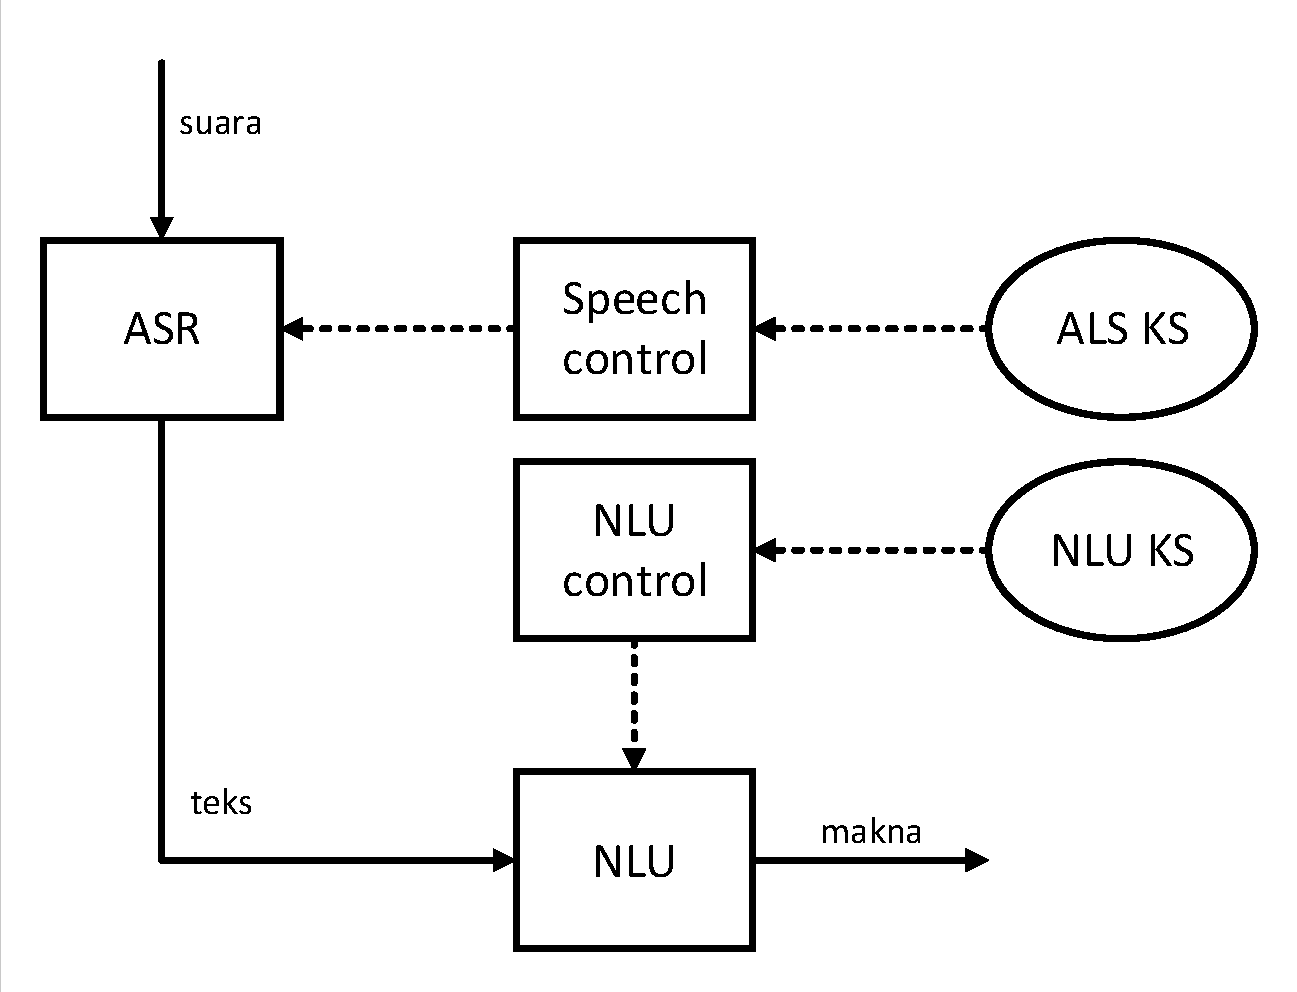
\includegraphics[width=0.5\textwidth, trim=2 2 2 2, clip]{resources/2/early_slu.pdf}
	\caption{Rancangan awal sistem SLU \parencite{tur2011spoken}}
	\label{fig:slu_early}
\end{figure}

Klasifikasi maksud kalimat berarti menentukan sebuah makna dari sebuah kalimat yang diberikan oleh pengguna. Sebagai contoh, kalimat “putarkan sebuah lagu” memiliki makna “putar media” berupa lagu. Makna tersebut kemudian diterjemahkan menjadi sebuah aksi oleh sistem. Makna kalimat bisa didapatkan dengan melihat kata-kata yang terkandung di dalam sebuah kalimat, atau melihat pola urutan kata dalam kalimat tersebut.

Pengisian slot adalah metode untuk mengambil entitas-entitas dari sebuah kalimat biasa. Beberapa aksi terkadang membutuhkan masukan parameter untuk melengkapi aksi tersebut. Masukan parameter didapatkan dari dalam kalimat yang dimasukkan oleh pengguna. Sebagai contoh, “putar lagu separuh aku dari noah” berarti pengguna menginginkan sebuah lagu diputarkan oleh sistem. Namun, permintaan pengguna menjadi lebih spesifik karena pengguna menyebutkan judul lagu beserta artis. Judul lagu adalah “separuh aku” dengan artis adalah “noah”. Metode yang dapat digunakan untuk mengambil entitas adalah melakukan pelabelan kata-kata yang menjadi entitas dengan menggunakan \textit{recurrent neural network} (RNN).

\section{\textit{Machine Learning}}

Pembelajaran mesin, atau \textit{machine learning}, adalah sebuah program komputer yang dirancang untuk belajar dari pengalaman dengan acuan berupa kelas tugas-tugas dan pengukuran performa, jika performa pada suatu tugas, yang telah diukur, diperbaiki dengan pengalaman \parencite{mitchell1997machine}. Pembelajaran mesin menggunakan data-data yang telah terkumpul untuk membentuk sebuah pola yang dapat digunakan pada data yang akan muncul atau dimasukkan oleh pengguna.

Pembelajaran mesin diterapkan pada berbagai macam aplikasi, yang ditujukan untuk mengurangi peran manusia dalam melakukan hal tersebut. Sebagai contoh, pembelajaran mesin digunakan untuk melakukan klasifikasi gambar, teks, suara, dan lain-lain. Selain itu, pembelajaran mesin diaplikasikan ke dalam analisis data dengan jumlah yang sangat besar atau biasa disebut sebagai \textit{big data}.

\section{\textit{Artificial Neural Network} (ANN)}

\textit{Artificial neural network} (ANN) adalah sistem komputasi yang memiliki elemen-elemen pemrosesan sederhana yang saling terhubung, yang mana dapat memproses informasi dengan respon keadaan dinamisnya kepada masukan dari luar \parencite{caudill1987neural}. Gambar \ref{} menggambarkan rupa dari ANN paling dasar. ANN terdiri dari tiga jenis lapisan, yaitu lapisan masukan, lapisan tersembunyi, serta lapisan keluaran. Lapisan masukan adalah lapisan yang berisi nilai-nilai masukan berasal dari data yang telah terkumpul. Lapisan tersembunyi berisi fungsi-fungsi aktivasi yang digunakan untuk menentukan keluaran yang diinginkan oleh \textit{neural network} secara keseluruhan.

\textit{Neural network} memiliki banyak variasi untuk kondisi data yang berbeda-beda. Jenis \textit{neural network} yang sangat dasar adalah \textit{feed forward neural network}, digunakan untuk melakukan klasifikasi sederhana. Untuk laporan ini, jenis \textit{neural network} yang digunakan adalah \textit{neural network} yang dapat digunakan dalam melakukan klasifikasi sekuensial, seperti \textit{recurrent neural network} (RNN) dan \textit{convolutional neural network} (CNN).

\section{\textit{Convolutional Neural Network} (CNN)}

\textit{Convolutional neural network} atau CNN biasa digunakan untuk mengenali objek-objek yang berada di dalam sebuah gambar. CNN mengambil sebidang area dengan ukuran yang telah ditentukan dalam sebuah gambar. Bidang tersebut digunakan secara berurutan, biasanya dari kiri ke kanan dan atas ke bawah, hingga seluruh gambar telah teridentifikasi. CNN mencoba memprediksi sebuah objek yang bersangkutan dengan mendeteksi fitur-fitur yang terdapat dalam sebuah gambar menggunakan \textit{filter}. Fitur tersebut didapatkan dengan cara melakukan \textit{dot product} pada bidang area gambar dengan \textit{filter}.

Untuk penerapan di dalam teks, fitur-fitur tersebut didapatkan dengan melakukan \textit{embedding} pada sebuah kata yang bersangkutan. \textit{Embedding} adalah proses untuk merepresentasikan sebuah kata menjadi vektor multi dimensi. Keuntungan yang dimiliki oleh CNN, jika dibandingkan dengan \textit{recurrent neural network} (RNN), adalah kemampuan CNN dalam melihat kata yang berada di depan satu kata yang sedang dilatih. Dengan begitu, CNN dapat mempertimbangkan kata sebelum dan kata selanjutnya untuk memasangkan label pada sebuah kata.

\section{\textit{Long Short Term Memory} (LSTM)}

\textit{Long short term memory} atau LSTM digunakan untuk mengatasi permasalahan latihan dengan menggunakan data yang bersifat \textit{sequential}. LSTM digunakan untuk mengatasi kelemahan yang dimiliki oleh RNN, yaitu RNN tidak mampu menyimpan informasi dalam jangka waktu yang sangat lama. LSTM dapat memutuskan apakah sebuah informasi akan diteruskan pada iterasi berikutnya atau dilupakan dengan bantuan dari gerbang pelupa (\textit{forget gate}).

Gambar \ref{fig:lstm} menunjukkan isi dari sebuah sel LSTM. Sel LSTM terdiri dari empat jenis gerbang, yaitu dua gerbang masukan, gerbang keluaran, dan gerbang pelupa. Semua gerbang mengandalkan masukan yang berasal dari masukan kata iterasi saat ini dan luaran dari iterasi sebelumnya. Kedua gerbang masuk mengolah nilai luaran dan masukan dengan menggunakan fungsi aktivasi sigmoid dan tanh, kemudian dilakukan operasi perkalian matriks pada kedua hasil tersebut. Gerbang pelupa mengolah kedua nilai dengan menggunakan fungsi aktivasi sigmoid. Terakhir, gerbang luaran mengolah kedua nilai dengan menggunakan fungsi aktivasi sigmoid. Kemudian terdapat sebuah nilai yang disebut dengan nilai keadaan sel. Nilai keadaan sel saat ini didapatkan dengan mengalikan nilai keadaan sel sebelumnya dengan nilai luaran gerbang pelupa, lalu ditambahkan dengan hasil dari kedua gerbang masukan.

\begin{figure}[H]
	\centering
	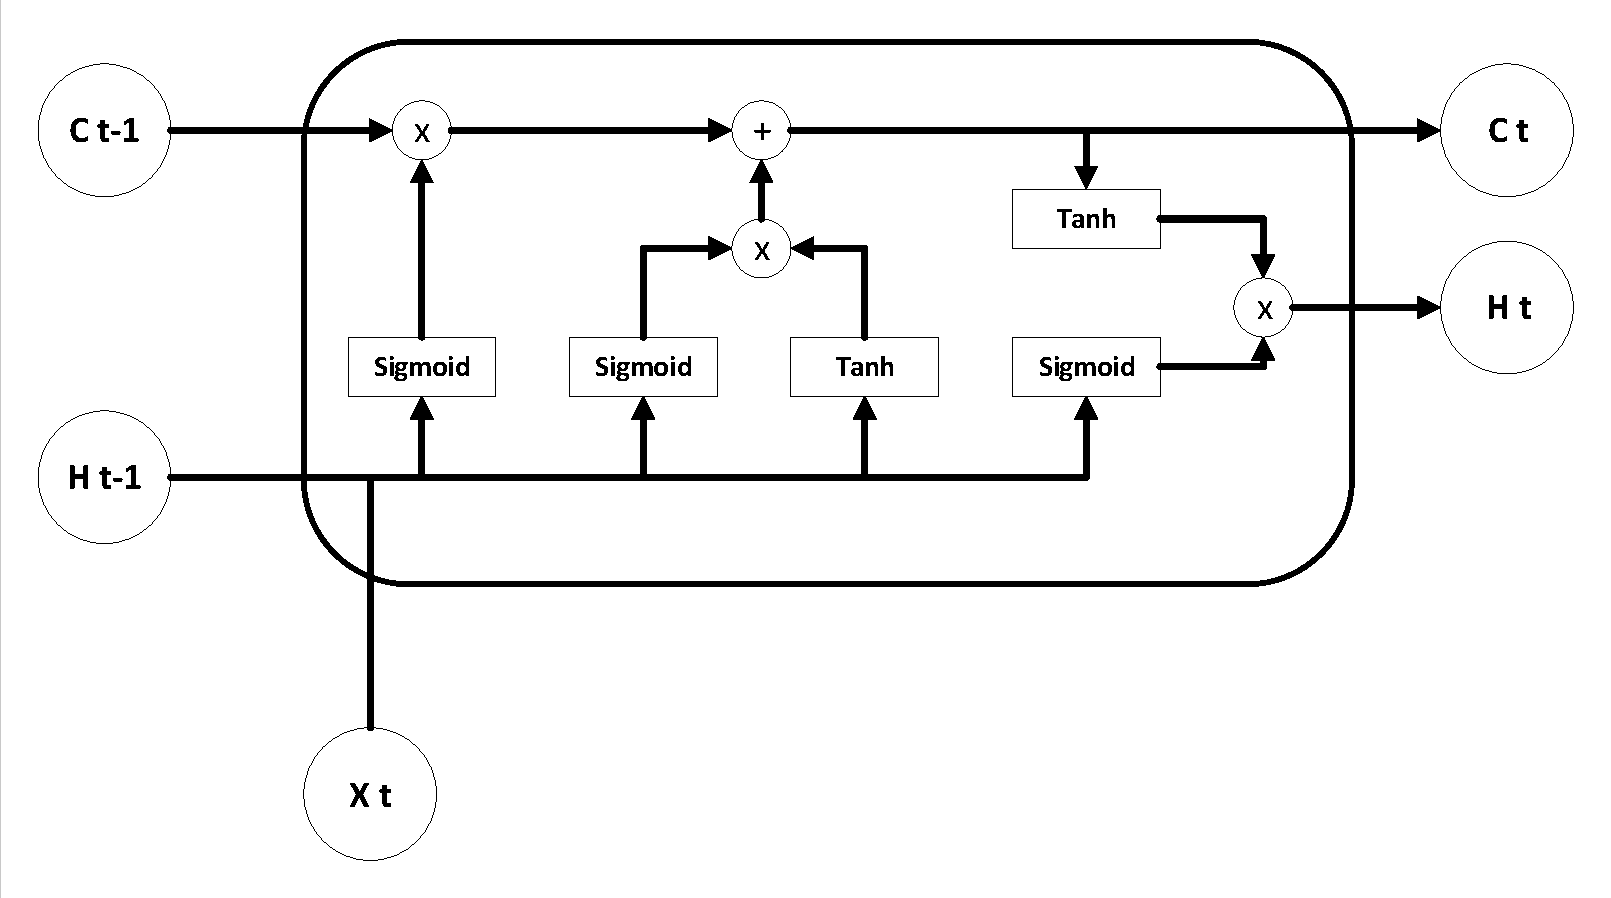
\includegraphics[width=0.8\textwidth, trim=2 2 2 2, clip]{resources/2/lstm.pdf}
	\caption{Arsitektur sel LSTM}
	\label{fig:lstm}
\end{figure}

\section{Analisis Produk}

Produk terkait yang menjadi acuan dalam pengerjaan Tugas Akhir adalah Rasa NLU, produk NLU \textit{open source} yang dibangun oleh Rasa HQ.

\subsection{Alat-Alat yang Digunakan}

Rasa NLU merupakan salah satu bagian dari Rasa Stack, \textit{library} Python yang digunakan untuk membangun sistem \textit{chatbot} berbasis NLU. Rasa NLU membutuhkan komponen-komponen sebagai berikut: spaCy sebagai \textit{library} pembantu Rasa NLU dalam melakukan pengolahan teks, dan fastText sebagai model vektor kata yang digunakan untuk membantu spaCy dalam mengolah teks.

\subsubsection{Rasa}

Rasa, terdiri dari Rasa NLU dan Rasa Core, adalah sepasang \textit{open-source library} Python yang digunakan untuk membangun perangkat lunak berbasis percakapan \parencite{bocklisch2017rasa}. Rasa biasanya digunakan untuk pengembangan robot percakapan atau dikenal dengan \textit{chatbot} berbentuk teks. Tujuan dari Rasa adalah membantu para pengembang untuk mengembangkan manajemen dialog dan pemahaman bahasa berdasarkan pembelajaran mesin. Pengembangan Rasa terinspirasi dari beberapa \textit{library} yang telah ada, seperti scikit-learn dan Keras untuk API, fastText untuk klasifikasi teks, dan GloVe untuk penyediaan data latih untuk \textit{word embedding}. Versi Rasa yang digunakan dalam pengerjaan Tugas Akhir, yaitu Rasa NLU versi 0.11.4 dan Rasa Core versi 0.8.6.

Arsitektur Rasa dapat dilihat pada Gambar \ref{fig:rasa_arch}. Terdapat empat bagian di dalam arsitektur Rasa, yaitu \textit{Interpreter, Tracker, Policy}, dan \textit{Action}. Bagian Interpreter ditangani oleh Rasa NLU, sedangkan bagian yang lain ditangani oleh Rasa Core. Rasa bersifat modular, sehingga \textit{library} dapat diintegrasikan dengan \textit{library} lain, seperti Rasa Core dapat dihubungkan dengan \textit{Interpreter} selain Rasa NLU, dan sebaliknya.

Tahap-tahap proses yang ada di dalam arsitektur Rasa dapat dijelaskan sebagai berikut. Pertama, pesan yang dimasukkan oleh pengguna dikirimkan ke \textit{Interpreter}. Di dalam \textit{Interpreter} dilakukan proses untuk mengekstrasi \textit{intent}, entities, dan beberapa informasi terstruktur lain dari pesan yang telah dimasukkan. Kedua, luaran dari \textit{Interpreter} diteruskan menuju \textit{Tracker}. \textit{Tracker} akan melacak \textit{state} dari percakapan dan memberikan pemberitahuan baru bahwa pesan telah diterima oleh \textit{Tracker}. Ketiga, \textit{Policy} menerima  \textit{state} dari \textit{Tracker}. Keempat, \textit{Policy} menentukan \textit{Action} yang harus dilakukan sebagai tanggapan pesan dari pengguna.Kelima, \textit{Action} yang terpilih dicatat oleh \textit{Tracker}. Terakhir, \textit{Action} mulai dieksekusi kepada pengguna, baik berupa pencarian atau mengeluarkan pesan.

\begin{figure}[H]
	\centering
	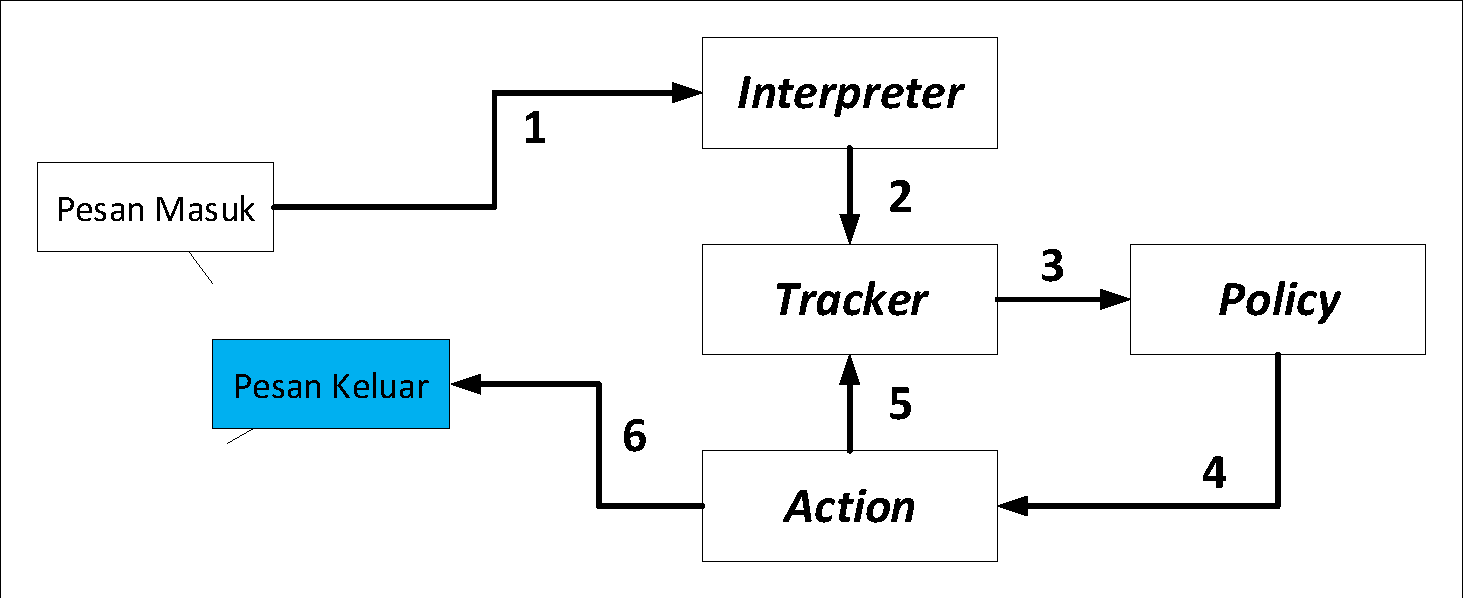
\includegraphics[width=0.9\textwidth, trim=2 2 2 2, clip]{resources/2/rasa_arch.pdf}
	\caption{Bagan arsitektur Rasa \parencite{bocklisch2017rasa}}
	\label{fig:rasa_arch}
\end{figure}

Secara sederhana, cara Rasa bekerja ditunjukkan oleh bagan pada Gambar \ref{fig:rasa_process}. Terdapat tiga proses utama dari Rasa NLU dan Rasa Core, yaitu melatih NLU, melatih dialog, dan menjalankan agen dialog.

\begin{figure}[H]
	\centering
	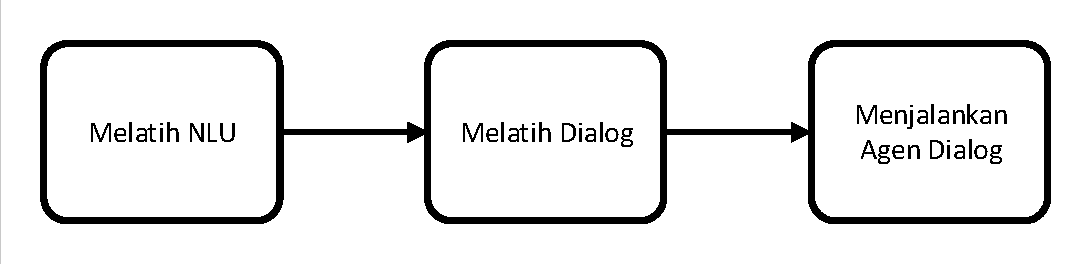
\includegraphics[width=0.8\textwidth, trim=2 2 2 2, clip]{resources/2/rasa_process.pdf}
	\caption{Bagan proses utama Rasa}
	\label{fig:rasa_process}
\end{figure}

\begin{enumerate}[label=\textit{\Alph*)}, itemindent=*, series=rasa_process_list]
	\item \textit{Melatih NLU}
\end{enumerate}

Pelatihan NLU dilakukan oleh Rasa NLU dengan bantuan pengolah teks seperti spaCy dan MITIE. Pelatihan NLU berguna untuk melatih sistem untuk dapat memahami teks dan entitas didalamnya yang akan dimasukkan oleh pengguna dan menyimpan model latihan untuk digunakan saat agen dialog siap untuk dijalankan.

Untuk dapat menjalankan proses ini, dibutuhkan dua data masing-masing dalam berbentuk file JSON, yaitu data latihan dan data konfigurasi. Data latihan berisi teks masukan yang dijadikan contoh, maksud dari teks tersebut, serta entitas yang terkandung di dalamnya. Sedangkan data konfigurasi berisikan konfigurasi yang digunakan sebagai acuan dalam melatih NLU, seperti bahasa, pipeline yang digunakan untuk latihan, lokasi data latihan, dan lain-lain.

Proses-proses untuk melatih NLU dapat dilihat pada Gambar \ref{fig:rasaNLU_train}, dan penjelasan tiap proses adalah sebagai berikut:

\begin{enumerate}
	\item Rasa NLU mengambil data konfigurasi, setelah itu mengambil data latihan,
	\item memuat data latihan dan mengubahnya menjadi obyek TrainingData,
	\item memuat data konfigurasi dan mengubahnya menjadi obyek RasaNLUConfig,
	\item membuat obyek Trainer sebagai “pelatih” dan mempersiapkan obyek tersebut dengan menggunakan obyek RasaNLUConfig sebagai masukan,
	\item memanggil prosedur latihan pada obyek Trainer dengan menggunakan obyek TrainingData sebagai masukan, dan,
	\item menyimpan model hasil latihan menuju direktori sistem.
\end{enumerate}

\begin{figure}[H]
	\centering
	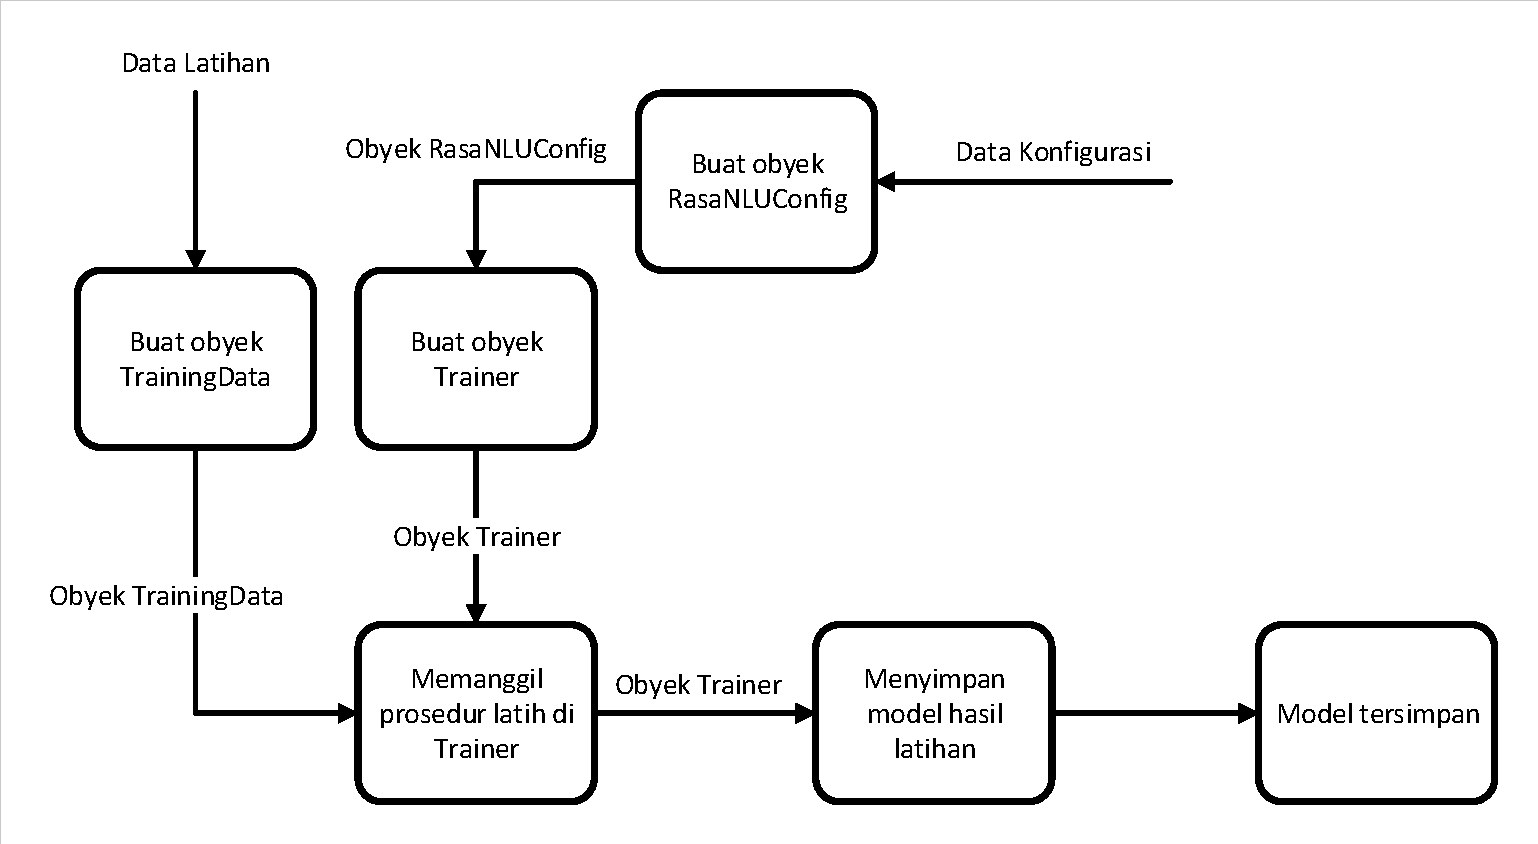
\includegraphics[width=0.8\textwidth, trim=2 2 2 2, clip]{resources/2/rasaNLU_train.pdf}
	\caption{Bagan alur latihan NLU dari Rasa NLU}
	\label{fig:rasaNLU_train}
\end{figure}

Di dalam data konfigurasi, terdapat pengaturan \textit{pipeline} yang digunakan untuk mengatur data latihan akan dilatih dengan menggunakan komponen apa saja. Alur persiapan \textit{pipeline} yang digunakan adalah, pertama menginisiasi semua komponen, lalu melakukan latihan jika terdapat prosedur latihan didalamnya, dan terakhir menyimpan hasil latihan per komponen ke dalam direktori sistem. Dalam pengerjaan Tugas Akhir ini, \textit{pipeline template} yang digunakan adalah spacy\_sklearn yang berisikan komponen latih sebagai berikut:

\begin{enumerate}
	\item nlp\_spacy, digunakan untuk inisialisasi spaCy sebelum menggunakan komponen latih spaCy yang lain,
	\item tokenizer\_spacy, digunakan untuk melakukan tokenisasi dari teks masukan dengan menggunakan tokenisasi dari spaCy,
	\item intent\_featurizer\_spacy, digunakan untuk membuat definisi ekstrasi fitur dari teks masukan dengan menggunakan spaCy. Fitur tersebut akan digunakan untuk melakukan klasifikasi maksud kalimat,
	\item intent\_entity\_featurizer\_regex, digunakan untuk mencatatkan seluruh \textit{regular expressio}n yang telah didefinisikan dalam data latihan,
	\item ner\_crf, digunakan untuk melakukan pengenalan entitas dengan menggunakan metode latihan \textit{conditional random field} (CRF) yang disediakan oleh \textit{library} sklearn-crfsuite,
	\item ner\_synonym, digunakan untuk menampung teks-teks yang memiliki nilai entitas yang sama, dan,
	\item intent\_classifier\_sklearn, digunakan untuk melakukan latihan klasifikasi maksud kalimat dengan masukan berupa fitur teks yang telah dilakukan oleh intent\_featurizer\_spacy. Latihan klasifikasi dilakukan dengan menggunakan \textit{support vector machine} (SVM) dan pengaturan parameter latih menggunakan metode \textit{grid-search} yang disediakan oleh scikit-learn.
\end{enumerate}

\begin{enumerate}[resume*=rasa_process_list]
	\item \textit{Melatih Dialog}
\end{enumerate}

Pelatihan dialog dilakukan dengan menggunakan Rasa Core. Pelatihan dialog berguna untuk mendefinisikan domain NLU dari sistem serta melatih agen dialog untuk menciptakan prediksi respon yang tepat berdasarkan masukan dari pengguna sebelumnya. Prediksi didapatkan dengan menggunakan sebuah komponen yaitu \textit{policy}.

Untuk dapat menjalankan proses ini, dibutuhkan dua data masing-masing dalam bentuk file \textit{markdown} dan YML, yaitu data cerita dan data domain. Data cerita digunakan untuk mengkonstruksi alur percakapan yang mungkin terjadi antara pengguna dengan sistem. Data cerita terdiri dari balok-balok cerita, berisi maksud kalimat yang diekstraksi dari teks masukan pengguna dan respon sistem terhadap masukan tersebut. Jumlah respon dan timbal balik dalam satu balok cerita tidak terbatas. Data domain digunakan untuk inisialisasi definisi dari maksud kalimat, entitas yang terlibat, slot yang tersedia, serta aksi yang akan dilakukan oleh sistem.

Proses-proses untuk melatih agen dialog dijelaskan sebagai berikut:

\begin{enumerate}
	\item Rasa Core mengambil data domain dan data cerita,
	\item membuat agen dialog dengan membuat obyek Agent menggunakan masukan data domain dan policy yang digunakan,
	\item memanggil prosedur latih dari obyek Agent dengan menyertakan data cerita sebagai masukan. Prosedur ini juga membuat obyek PolicyTrainer dan melakukan pelatihan, dan,
	\item menyimpan agen dialog terlatih ke dalam direktori sistem.
\end{enumerate}

\begin{enumerate}[resume*=rasa_process_list]
	\item \textit{Menjalankan Agen Dialog}
\end{enumerate}

Setelah model NLU dan agen dialog telah tersimpan ke dalam direktori, sistem sudah siap untuk menjalankan agen dialognya. Sistem akan melakukan \textit{loop} selamanya terhadap proses memasukkan teks. Teks yang telah dimasukkan oleh pengguna akan diprediksi maksud kalimatnya sehingga sistem dapat menentukan aksi yang tepat.

\subsubsection{spaCy}

spaCy adalah sebuah \textit{open-source library} Python digunakan untuk melakukan pengolahan teks, khususnya NLP, dalam tingkat industri \parencite{spacy2}. spaCy mendukung banyak bahasa selain MITIE, dan lebih mudah untuk menambahkan bahasa baru, cukup dengan menyediakan model bahasa yang dibutuhkan ke dalam spaCy. Versi spaCy yang digunakan adalah versi 2.0.11.

Arsitektur spaCy dapat terlihat di dalam Gambar \ref{fig:spaCy_arch} \parencite{spacy2}. Terdapat dua struktur data pusat yang berada di dalam spaCy, yaitu Doc dan Vocab. Doc berisi rangkaian dari \textit{token} dan semua anotasinya, sedangkan Vocab berisi sekumpulan tabel \textit{look-up} untuk menyediakan informasi umum ke seluruh dokumen, bertujuan untuk mencegah terjadinya duplikasi data dan memastikan bahwa fakta hanya tersimpan di dalam satu sumber.

Dengan menyimpan semua fakta di dalam satu sumber dapat menghemat penyimpanan di dalam arsitektur spaCy itu sendiri. Seperti, Doc menyimpan seluruh data-data anotasi teks, sedangkan Token dan Span hanya berupa \textit{view} yang berisi \textit{pointer} untuk merujuk kepada data yang ada di Doc.

\begin{figure}[H]
	\centering
	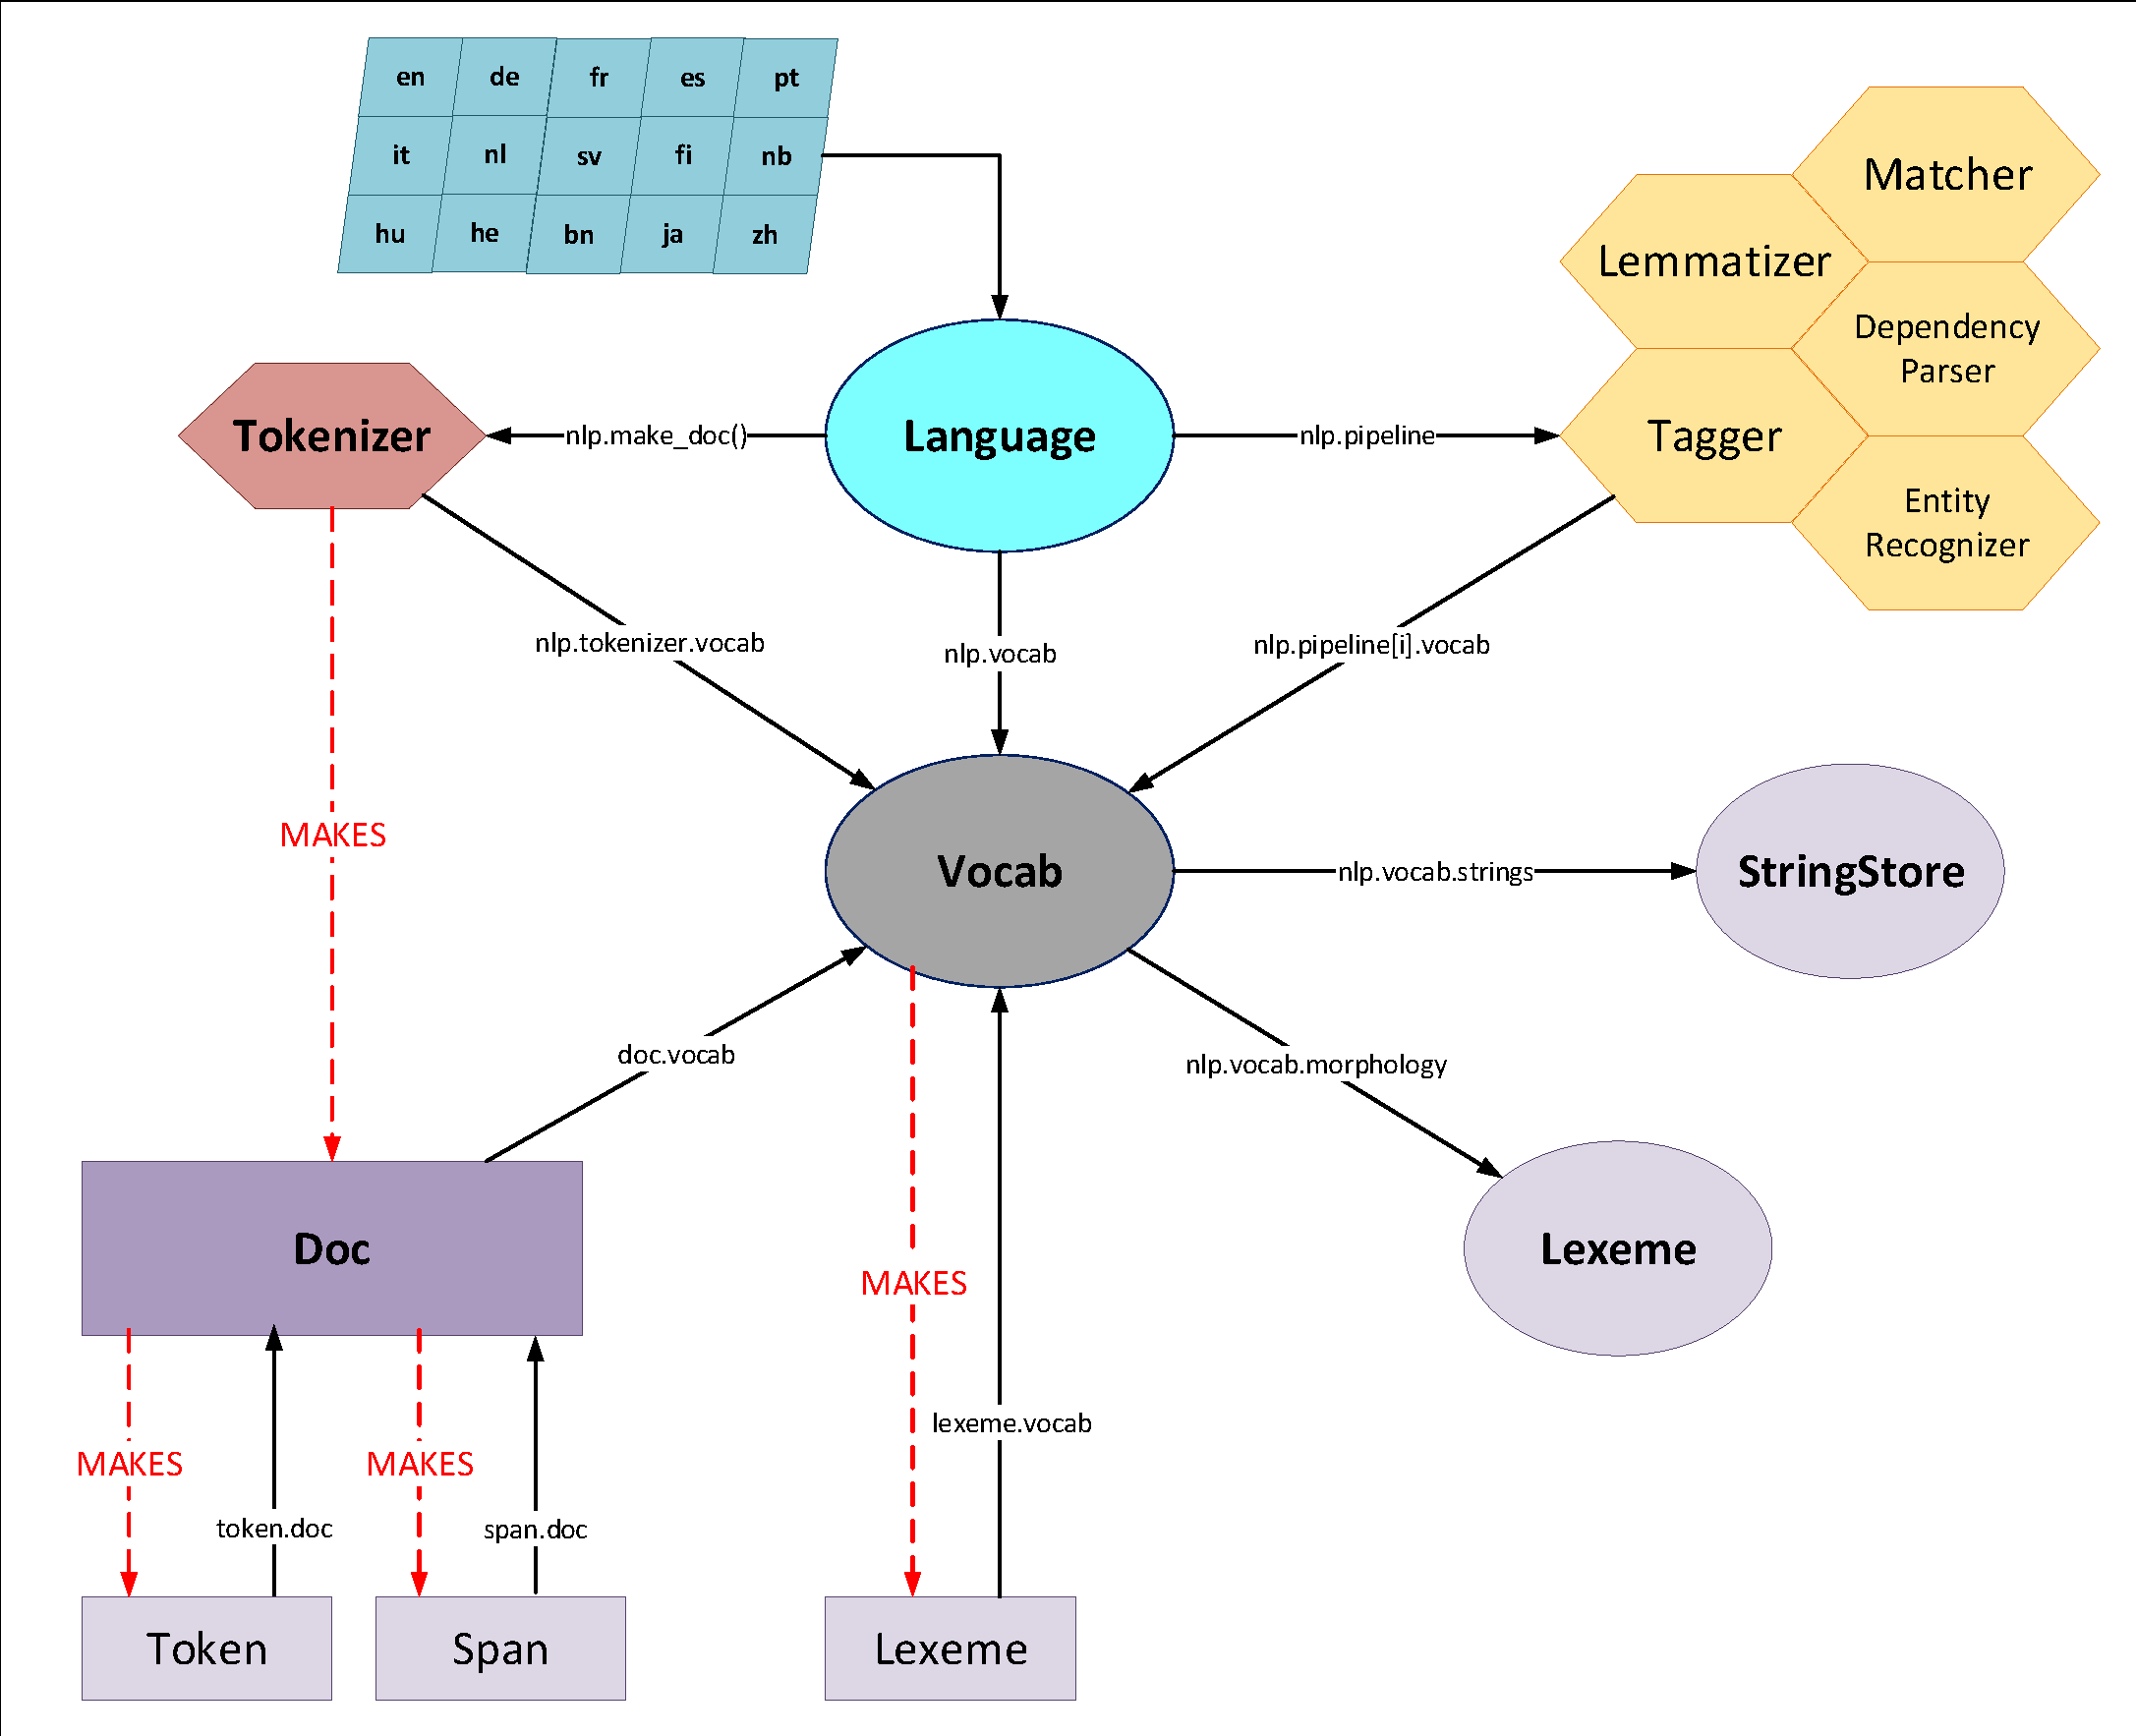
\includegraphics[width=0.9\textwidth, trim=2 2 2 2, clip]{resources/2/spacy_arch.pdf}
	\caption{Bagan arsitektur spaCy \parencite{spacy2}}
	\label{fig:spaCy_arch}
\end{figure}

\subsubsection{fastText}

fastText adalah \textit{library} untuk klasifikasi dan representasi teks yang dibangun oleh peneliti AI dari Facebook \parencite{joulin2017bag}. Pemrosesan yang dilakukan adalah mengubah sebuah kalimat-kalimat yang tersedia menjadi sebuah model vektor. Model vektor merepresentasikan kedekatan antara suatu kata dengan kata yang lain, memiliki nilai rentang antara 0 hingga 1. Model vektor tersebut dapat dipakai tidak hanya oleh \textit{library} fastText, namun juga dapat digunakan oleh \textit{library} luar, seperti spaCy.

Untuk pengerjaan Tugas Akhir ini, digunakan model vektor yang telah tersedia oleh fastText di dalam repositori GitHub. Model vektor yang digunakan adalah model vektor berbahasa Indonesia, yang diproses dari teks-teks yang tersedia di Wikipedia. Untuk dapat menggunakan model vektor, terlebih dahulu model vektor dikonversi menjadi model bahasa spaCy, dalam hal ini model bahasa Indonesia.

\subsection{Teori yang Diterapkan}

\subsubsection{Pengenalan Entitas dengan \textit{Conditional Random Field}}

\textit{Conditional random field} (CRF) adalah metode pembelajaran yang digunakan untuk data-data yang bersifat berurutan. CRF menggunakan fitur-fitur yang dimiliki oleh sebuah kata untuk melakukan pelatihan. Fitur yang digunakan untuk CRF dapat bervariasi sesuai kebutuhan, namun fitur dasar yang tersedia adalah kata utama dan kata sebelum kata utama. CRF biasanya digunakan untuk \textit{sequence labelling} teks.

Rasa NLU menggunakan \textit{library} Python yaitu sklearn-crfsuite. \textit{Library} ini merupakan pembungkus \textit{library} python-crfsuite yang mana menyediakan \textit{estimator} yang cocok dengan scikit-learn \parencite{sklearncrf}. Hal tersebut memudahkan penggunaan model CRF untuk pelatihan dan menyimpan model hasil latihan. Selain itu, spaCy juga menyediakan fitur yang dapat digunakan oleh CRF milik Rasa NLU, yaitu fitur POS \textit{tag} untuk tiap kata dalam kalimat.

\subsubsection{Klasifikasi Maksud Kalimat dengan \textit{Support Vector Machine}}

\textit{Support vector machine} (SVM), atau \textit{support vector network}, adalah sebuah metode pembelajaran yang memetakan vektor masukan menjadi ruang fitur dengan dimensi yang tinggi melalui pemetaan non linear yang telah dipilih sebelumnya \parencite{cortes1995support}. SVM biasanya digunakan untuk menjelaskan kegiatan klasifikasi dengan metode support vector, namun kegunaan SVM juga bisa digunakan untuk kegiatan regresi. Oleh karena itu, SVM terbagi menjadi dua, yaitu \textit{support vector classification} (SVC) untuk klasifikasi dan \textit{support vector regression} (SVR) untuk regresi \parencite{gunn1998support}.

Rasa NLU menggunakan SVM untuk melakukan klasifikasi maksud kalimat dari scikit-learn. Dengan jumlah maksud kalimat yang berjumlah lebih dari dua, maka scikit-learn akan menggunakan metode-metode untuk mengakali SVM sehingga dapat digunakan untuk kasus melakukan klasifikasi lebih dari dua kelas. Selain itu, Rasa menggunakan metode \textit{grid-search} untuk melakukan \textit{hyperparameter tuning.}

\subsection{Analisis Kekurangan Sistem}

Selama pengerjaan sistem NLU berlangsung, terdapat kekurangan-kekurangan yang dimiliki oleh alat-alat yang digunakan untuk membangun sistem. Kekurangan tersebut berkaitan dengan permasalahan proyek yang sedang dikerjakan.

\subsubsection{Model yang Digunakan Tidak Cukup}

Model vektor fastText digunakan untuk dapat membangun model bahasa Indonesia spaCy, dan digunakan dalam melakukan pengolahan teks di Rasa. Namun, model bahasa yang berhasil dibangun dari model vektor hanyalah pada bagian kosakata saja. Untuk dapat membangun sistem Rasa NLU yang baik, model juga memerlukan bagian \textit{tagger} untuk diberikan kepada sistem CRF.

%\textit{Named entity recognition}, atau NER, merujuk kepada pengenalan \textit{token-token} yang merupakan sebuah entitas, seperti nama oganisasi, nama tempat, tanggal, waktu, angka urutan, dan lain-lain. NER diperlukan untuk membedakan antara \textit{token} biasa dengan \textit{token} entitas. \textit{Parser} merujuk kepada \textit{dependency parsing} yaitu melihat ketergantungan sebuah token dengan token yang lain. Sebagai contoh, kalimat “Budi memakan nasi” memiliki dua ketergantungan, yaitu “Budi” memiliki ketergantungan subyek dengan “memakan”, dan “nasi” memiliki ketergantungan obyek dengan “memakan”. Terakhir, \textit{tagger} merujuk kepada \textit{POS tagging} yaitu memberikan tanda kepada token berdasarkan sifat kata dari token tersebut, misal kata kerja, kata benda, tanda baca, dan lain-lain.
%
%Terdapat beberapa korpus untuk latihan yang menyediakan komponen seperti \textit{dependency parser} dan \textit{POS tag}, salah satunya berasal dari Universal Dependencies. Universal Dependencies menyediakan korpus yang diambil dari berbagai sumber, seperti berita, artikel blog, istilah hukum, istilah medis, Wikipedia, dan lain-lain.
%
\subsubsection{Kebutuhan Ekstraksi Fitur untuk CRF}

CRF membutuhkan fitur-fitur yang telah didefinisikan sebelumnya untuk dapat melakukan latihan, seperti CRF yang diterapkan oleh Rasa membutuhkan fitur POS \textit{tag} pada sebuah kata. Fitur tersebut hanya bisa didapatkan dengan \textit{library} NLP, seperti spaCy, yang dapat melakukan latihan POS \textit{tag} berdasarkan model yang telah disediakan oleh pengguna. Oleh karena itu, sebuah kalimat masukan perlu melakukan klasifikasi dengan spaCy terlebih dahulu sebelum akhirnya diekstraksi dengan menggunakan Rasa.

Model vektor fastText digunakan untuk dapat membangun model bahasa Indonesia spaCy, dan digunakan dalam melakukan pengolahan teks di Rasa. Namun, model bahasa yang berhasil dibangun dari model vektor hanyalah pada bagian kosakata saja. Untuk dapat membangun model bahasa yang baik, model juga memerlukan bagian-bagian seperti POS \textit{tagger}. Kekurangan informasi tersebut berakibat pada klasifikasi spaCy yang menjadi tidak maksimal.

Lalu, model dari fastText hanya tersedia dalam bahasa Indonesia yang baku. Hal ini dapat menyebabkan kesulitan dalam mengenal kata-kata yang baru diucapkan, atau kata yang tidak baku seperti kata-kata dalam percakapan sehari-hari. Oleh karena itu, pendekatan CRF dari Rasa NLU tidak cocok untuk digunakan pada proyek ini.

%\subsubsection{Penggunaan SVM untuk Klasifikasi Lebih dari Dua Kelas}
%
%Rasa NLU menggunakan metode SVM dengan tambahan pengaturan grid-search dari scikit-learn untuk melakukan pelatihan klasifikasi maksud kalimat. Kelemahan yang terdapat pada SVM dalam melakukan klasifikasi adalah SVM hanya dapat melakukan klasifikasi pada dua kelas saja. SVM tidak dirancang untuk mengatasi permasalahan klasifikasi yang membutuhkan lebih dari dua kelas. Namun, scikit-learn dapat mengatasi permasalahan tersebut dengan menggunakan skema klasifikasi one-versus-one. Skema tersebut bekerja dengan cara membuat satu alat klasifikasi untuk tiap pasangan kelas yang ada. Pada saat prediksi, kelas yang menerima voting tertinggi akan terpilih [cit].
%
%Kelemahan yang dimiliki oleh skema one-versus-one adalah jumlah klasifikasi yang dilakukan, yaitu (jumlah kelas * (jumlah kelas – 1) / 2) klasifikasi, membuat skema ini memiliki kompleksitas O(jumlah kelas \^{} 2). Dengan jumlah klasifikasi yang banyak, SVM dirasa tidak efisien untuk melakukan klasifikasi dengan jumlah kelas yang banyak. Oleh karena itu, metode klasifikasi yang tepat digunakan untuk mengatasi masalah jumlah kelas lebih dari dua tersebut adalah \textit{neural network}.
%
%Keluaran dari \textit{neural network} dapat diatur sesuai dengan jumlah kelas yang tersedia pada data latihan. Fleksibilitas yang dimiliki oleh \textit{neural network} membuat metode ini dapat melakukan satu model dan satu kali latihan klasifikasi untuk dapat menghasilkan model yang bagus untuk digunakan.
\end{comment}